\documentclass[twoside,11pt]{article}
\usepackage{amsmath,amsfonts,amssymb,amsthm}
\usepackage{graphicx,color}
\usepackage{verbatim,url}
\usepackage{listings}
\usepackage{upquote}
\usepackage[T1]{fontenc}
%\usepackage{lmodern}
\usepackage[scaled]{beramono}
%\usepackage{textcomp}
\usepackage{ifthen}

% Directories for other source files and images
\newcommand{\bibtexdir}{../bib}
\newcommand{\figdir}{eps}

\newcommand{\E}{\mathrm{E}}
\newcommand{\Var}{\mathrm{Var}}
\newcommand{\N}{\mathcal{N}}
\newcommand{\matlab}{{\sc Matlab}\ }

\setlength{\textheight}{9in} \setlength{\textwidth}{6.5in}
\setlength{\oddsidemargin}{-.25in}  % Centers text.
\setlength{\evensidemargin}{-.25in} %
\setlength{\topmargin}{0in} %
\setlength{\headheight}{0in} %
\setlength{\headsep}{0in} %

\renewcommand{\labelenumi}{(\alph{enumi})}
\renewcommand{\labelenumii}{(\arabic{enumii})}

\theoremstyle{definition}
\newtheorem{MatEx}{M{\scriptsize{ATLAB}} Usage Example}

\definecolor{comments}{rgb}{0,.5,0}
\definecolor{backgnd}{rgb}{.95,.95,.95}
\definecolor{string}{rgb}{.2,.2,.2}
\lstset{language=Matlab}
\lstset{basicstyle=\small\ttfamily,
        mathescape=true,
        emptylines=1, showlines=true,
        backgroundcolor=\color{backgnd},
        commentstyle=\color{comments}\ttfamily, %\rmfamily,
        morecomment=[l]{\%},
        morecomment=[is]{\%\#}{\%\#},
        stringstyle=\color{string}\ttfamily,
        keywordstyle=\ttfamily, %\normalfont,
        showstringspaces=false}
\newcommand{\matp}{\mathbf{\gg}}

\newcommand{\myraise}{\vspace{-.15cm}}

\raggedbottom
\begin{document}
\clearpage
\thispagestyle{empty}
\centerline{\Large {\bf Team DAB: } CS74/174 Homework \#3}
\centerline{Machine Learning and Statistical Data Analysis: Winter 2016}
\centerline{{\bf D}aniel Chen, {\bf A}ndrew Kim, {\bf B}enjamin Packer}
% \vspace{1cm}

% Your team will produce a single write-up PDF document, approximately 6 pages long, and less than 8 pages. You report will describe the problem you chose to tackle and the methods you used to address it, including which model(s) you tried, how you trained them, how you selected any parameters they might require, and how they performed in on the test data. Consider including tables of performance
% of different approaches, or plots of performance used to perform model selection (i.e., parameters that control complexity). Please report your leaderboard result in your report as well.
% You are free to collaborate with other teams, including sharing ideas and even code, but please document where your predictions came from. For example, for any code you use, please say in your report who wrote the code and how it was applied (who determined the parameter settings and how, etc.) Collaboration is particularly true for learning ensembles of predictors: your teams may each supply a set of predictors, and then collaborate to learn an ensemble from the set.

% You need to submit your pdf report; without it, you can not get grades.
% You do not need to submit your code, but if you want to, please put your code in a separate zip file).
% It is like submitting an academic paper: you can submit any supplementary documents as you want, but your main paper should be self-contained and include all the information for the readers to understand your story and your results.
% In addition, I'm sure Prof. Liu mentioned in class that the project report is due Monday, March 14th at 11:59pm.

\tableofcontents
\newpage
\clearpage
\setcounter{page}{1}

\section{Introduction}
  % overview of the problem
  % what we did

  This project worked on finding a solution to the BNP Paribas Cardif Claims Management Kaggle competition. The competition is to use machine learning algorithms to effectively classify claims with anonymized data into two classes with minimal error:

  \begin{enumerate}
    \item claims for which approval could be accelerated leading to faster payments
    \item claims for which additional information is required before approval
  \end{enumerate}

  The purpose of this classification is to allow BNP Paribas Cardif to accelerate its claims process and provide a better service to its customers.

  Error on both Kaggle and as presented in this paper is measured through Log Loss:

  \[ \text{logloss} = - \frac{1}{N} \sum\limits_{i=1}^N (y_i \log(p_i) + (1 - y_i) \log(1 - p_i)) \]

  $N$ is the number of observations, $log$ is the natural log, $y_i$ is the binary target and $p_i$ is the predicted probability that $y_i = 1$

  In the end, our solution is a ensemble of logistic regression, neural networks, and boosted trees. Our best testing error is XXXX, which ranks XXXX on the leaderboard.

\section{The Data}
  % overview of the data

  The data given is split into training and testing. The sets are the same, except we do not know the expected targets on the testing data (Kaggle retains this information to prevent cheating).

  The training set consists of 114,321 examples while the test set contains 166,607. Each example consists of 131 features, 19 which are categorical with the remaining numerical. The features are all anonymized, so we don't know what the data means.

  \subsection{Analysis of the Data}
    % we could discuss this?
    % https://www.kaggle.com/bobcz3/bnp-paribas-cardif-claims-management/exploring-bnp-data-distributions/notebook
    % we could also do feature selection. or we could remove the section altogether, idk

  \subsection{One Hot Encoding}
    % Daniel will cover this
    We originally converted our categorical features to integer values. This confused our classifiers into believing the features expressed a numerical relationship. By switching over to a one-hot-encoding of our categorical features, we were able to improve performance.

    One-hot-encoding splits each feature into $n$ features, where $n$ is the number of unique values that this feature takes on in both the training and testing sets. Each of these resulting features either take on 0 or 1. For each data point, only a single feature (the one which corresponds to the value that the original categorical feature had) has the value 1. This increases the number of features, but allows for correct encoding of categorical data.

    One issue with one-hot-encoding was that we had to remove one of the categorical features, v22. This is because this feature had over 1000 unique values, so it increased the number of features to a number which was computation cumbersome. We prefer the empirical increase in performance to the loss of this single feature.

    Our original logistic regression without one hot encoding achieved an error of 0.49859. After switching to one-hot-encoding our error significantly to 0.48213.
    
  \subsection{Missing Values}
    There was lots of missing data in both the testing and training sets, which was a problem for both our Logistic Regression classifier and our Neural Networks, which XGBoost could handle missing values. Our first intuition was to impute each missing data value with the mean value for each feature, which seemed to work well. 

    However, we also experimented with setting the missing values to the median and mode of the missing data. Go on with results...

\section{Logistic Regression}
  Logistic regression was implemented using SciKit Learn's Logistic Regression classifier, which can output a probability for a given value. It allows specification of the $C$ parameter, which is equivalent to $\frac{1}{\alpha}$, where $\alpha$ is the regularization parameter.

  \subsection{Logistic Regression Parameter Tuning}
  Given a simple logistic regression model, the main parameter available to us for tuning was $\alpha$, or the regularization parameter. To find the optimal value for $\alpha$, we used 5-fold cross validation to as the objective function, and selected the $\alpha$ that best minimized it. The result was $\frac{1}{\alpha} = $, which is a slight regularization.

  \subsection{Performance and Final Selection}



\section{Boosted Trees}
  % Daniel will cover this

  Following suggestions on the forum, we implemented boosted trees using the XGBoost library, which stands for eXtreme gradient boosting. The library is designed and optimized for boosted tree algorithms. We utilized the Python package for this library. The classifier uses an ensemble of trees.

  The seven parameters that we optimize are shown below:

  % http://www.analyticsvidhya.com/blog/2016/03/complete-guide-parameter-tuning-xgboost-with-codes-python/
  \begin{description}
    \item[max\_depth] The maximum depth of a tree in the ensemble
    \item[min\_child\_weight] Defines the minimum sum of weights of all observations required in a child
    \item[gamma] The minimum loss reduction required to make a split
    \item[colsample\_bytree] The fraction of columns to be randomly sampled for each tree
    \item[subsample] The fraction of observations to be randomly samples for each tree
    \item[eta] The learning rate
    \item[num\_rounds] The number of rounds
  \end{description}

  \subsection{XGBoost Parameter Tuning}
    The parameters were tuned using two-fold cross validation. After playing around with tuning the parameters manually, we ran two large sets of parameters in an attempt to reduce error and understand the empirical relationships between the parameters.

    \subsubsection{Tuning 1}
      The first optimization iterated through all 120 combinations of these parameters:

      \begin{lstlisting}
max_depths = [2, 3, 4, 5, 6]
min_child_weights = [1]
gammas = [0, 1]
colsample_bytrees = [0.5, 1]
subsamples = [0.5, 1]
rounds_and_eta = [(20, 0.3), (50, 0.1), (100, 0.05)]
      \end{lstlisting}

      With this, our best results are shown below:

      \begin{center}
          \begin{tabular}{ | l | l | l | l | l | l | l | l | p{5cm} |}
          \hline
          error & runtime & minchildweight & subsample & eta & colsamplebytree & max depth & gamma \\ \hline
          0.468638593 & 347.661603 & 1 & 1 & 0.05 & 0.5 & 6 & 0 \\ \hline
          0.468680062 & 346.063396 & 1 & 1 & 0.05 & 0.5 & 6 & 1 \\ \hline
          0.468846706 & 177.2962441 & 1 & 1 & 0.1 & 0.5 & 6 & 1 \\ \hline
          0.468898392 & 178.4002779 & 1 & 1 & 0.1 & 0.5 & 6 & 0 \\ \hline
          0.469002588 & 661.6131201 & 1 & 1 & 0.05 & 1 & 6 & 1 \\ \hline
          \end{tabular}
      \end{center}

      The testing error found using the best parameters from the tuning was: 0.46853

    \subsubsection{Tuning 2}

      Our second optimization iterated through all 24 combinations of these parameters:

      \begin{lstlisting}
max_depths = [6, 8, 10]
min_child_weights = [1, 2]
gammas = [0]
colsample_bytrees = [0.5, 1]
subsamples = [1]
rounds_and_eta = [(200, 0.05), (300, 0.01)]
      \end{lstlisting}

      With this, our best results are shown below:

      \begin{center}
          \begin{tabular}{ | l | l | l | l | l | l | l | l | p{5cm} |}
          \hline
          error & runtime & minchildweight & subsample & eta & colsamplebytree & max depth & gamma \\ \hline
          0.464182985 & 1191.265073 & 1 & 1 & 0.05 & 0.5 & 10 & 0 \\ \hline
          0.464419596 & 1154.138998 & 2 & 1 & 0.05 & 0.5 & 10 & 0 \\ \hline
          0.46442771 & 959.313591 & 2 & 1 & 0.05 & 0.5 & 8 & 0 \\ \hline
          0.464540668 & 1020.961268 & 1 & 1 & 0.05 & 0.5 & 8 & 0 \\ \hline
          0.466287292 & 760.0540562 & 2 & 1 & 0.05 & 0.5 & 6 & 0 \\ \hline
          \end{tabular}
      \end{center}

      The testing error found using the best parameters from this tuning was: 0.47856

      Since this testing error is greater than the testing error achieved from the first tuning, there is evidence that somewhere between the first tuning and the second tuning we began to overfit the training data.

    \subsubsection{Final Selection of Parameters to be Ensembled}

      Although we did not end up using the optimal results from our tuning, it provided valuable insights to how we can use the parameters to achieve better results. Ultimately the results from our tuning was leading us to areas where this kind of brute force technique towards parameter tuning would become too computationally expensive, as tuning 2 already took nearly 12 hours to run.

      Mostly we spent time modifying eta, max\_depth, and colsample\_bytree.

      Ultimately, the parameters that we came up with were:
      \begin{lstlisting}
max_depths = 16
min_child_weights = 1
gammas = 0
colsample_bytrees = 0.68
subsamples = 0.5
num_round = 1800
eta = 0.01
      \end{lstlisting}

      This gave us a testing error of 0.45695 and the training was 0.286874075363. The runtime was approximately 4 hours.

\section{Neural Networks}
The Kaggle forums indicated that there was not much success using neural networks for this dataset. However, we attempted to build neural network models to help build the ensemble and to gain experience building neural nets. We trained a variety of different neural network architectures using the Theano Python libraries. We also used Lasagne which is a module built on top of Theano. All of the neural network structures has 498 input units and 2 output units. The 2 output units are softmax units, which have output between 0 and 1. We used rectified linear units (ReLU) in the hidden layer because we trained deep neural networks, which works well with ReLU. \cite{ReLU}

\subsection{One-Layer Network}
We first trained two-layer networks. We tested different numbers of units in the hidden layer. Since there are 498 input features, the first layer has 498 units and there are two output units. We read online that it is generally better to normalize the input data before feeding it into the network, so we normalized the data. We used 80\% of the training data for training and cross-validated on 20\% of the data. The picture below is a picture of the terminal output when training the neural network. The lasagne package prints out its own values for cross-validation and training error each epoch as it trains itself on the training dataset. You can see that we should have stopped training the neural network after epoch 14 since the cross-validation error consistently when up after that epoch, meaning that the network started to overfit. At the end of training, the python script prints out the log-loss error on the cross-validation set. 

      \begin{center}
        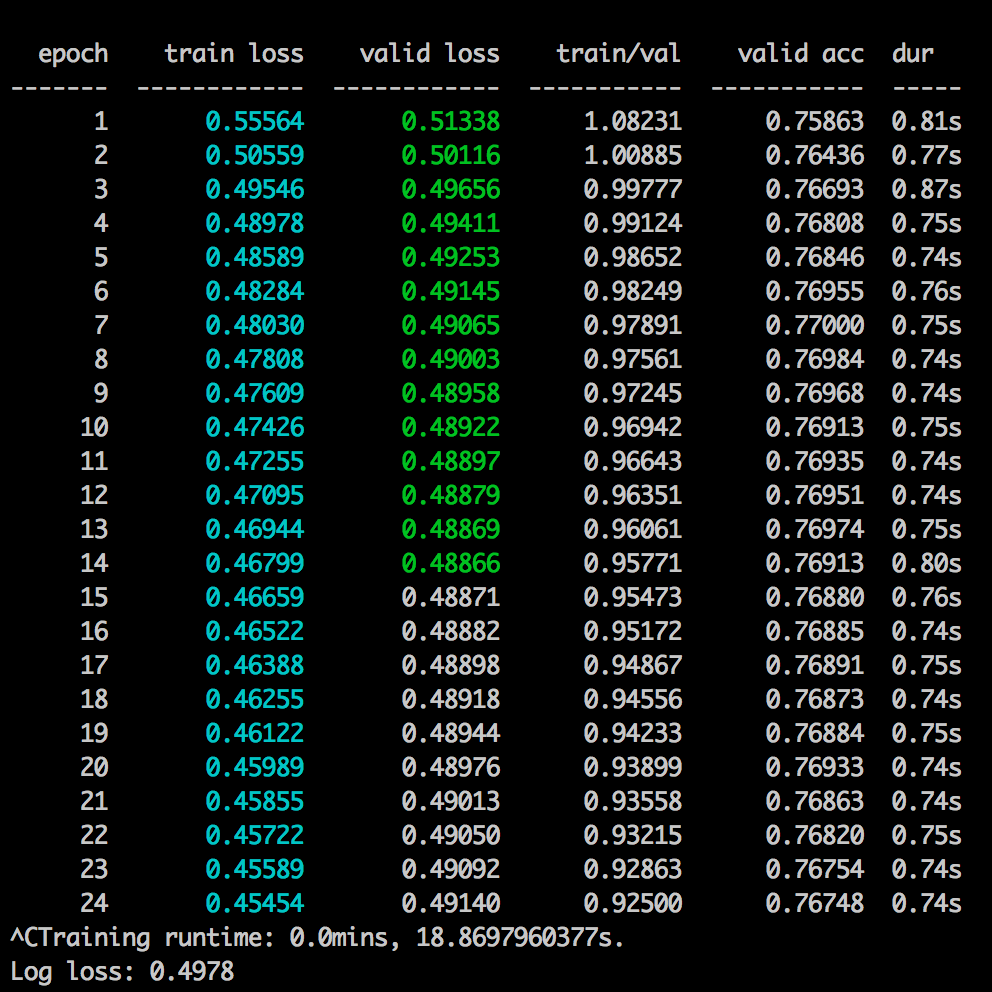
\includegraphics[scale=0.45]{nn1.jpg}
      \end{center}  

Below are the results for different numbers of hidden units. As you can see, all three networks are clearly overfitting since the cross-validation error is higher than the training error. Therefore, we took steps to try to address this issue. 

      \begin{center}
          \begin{tabular}{ | l | l | l | l | p{5cm} |}
          \hline
          Hidden Units & cv log-loss & training log-loss & epochs \\ \hline
          150 & 0.4978 & 0.45454 & 25 \\ \hline
          100 & 0.493 & 0.46028 & 25 \\ \hline
          50 & 0.4923 & 0.46281 & 25 \\ \hline 
          \end{tabular}
      \end{center}

\subsection{Dropout}
In order to prevent overfitting, we implemented a neural network with dropout layers. Though dropout is a technique particularly useful for deep neural networks, we tried the dropout layers to see its effect. Dropout prevents neural networks from overfitting by randomly dropping units and their connections with a probability, p.\cite{Dropout} The results are below for the same networks as above with dropout implemented in the hidden layer with probability of dropout set to 0.5. Including dropout causes the training error to decrease more slowly, but the the cross-validation error decreased for all three networks. 

      \begin{center}
          \begin{tabular}{ | l | l | l | l | p{5cm} |}
          \hline
          Hidden Units & cv log-loss & training log-loss & epochs \\ \hline
          150 & 0.4844 & 0.47525 & 100 \\ \hline
          100 & 0.4845 & 0.47909 & 100 \\ \hline
          50 & 0.4831 & 0.47761 & 100 \\ \hline 
          \end{tabular}
      \end{center}

\subsection{Two-Layer Network}
Rather than implementing PCA for feature selection and then using those features as input to the 1-hidden layer network, we tried implementing a two-layer network because deep neural networks select the relevant features itself. We used dropout in both layers because when testing with dropout in only one layer, overfitting occurred. The probability in the dropout layers was set to 0.5, the default value. 

      \begin{center}
          \begin{tabular}{ | l | l | l | l | p{5cm} |}
          \hline
          Layer 1 Hidden Units & Layer 2 Hidden Units & cv log-loss & training log-loss & epochs \\ \hline
          200 & 50 & 0.4806 & 0.48322 & 100 \\ \hline
          150 & 100 & 0.4854 & 0.48089 & 100 \\ \hline
          150 & 50 & 0.4824 & 0.48540 & 100 \\ \hline
          150 & 20 & 0.4870 & 0.48982 & 100 \\ \hline
          100 & 50 & 0.4866 & 0.48389 & 100 \\ \hline
          100 & 20 & 0.4924 & 0.48718 & 100 \\ \hline
          \end{tabular}
      \end{center}

As you can see in the results, we achieved the lowest cross-validation error with the neural network with 200 hidden units in the first layer and 50 units in the second layer. What was interesting was that the training log-loss error was higher than the cross-validation error for some networks. This may be because the validation set contains data that is \"easier\" to predict. 

\subsection{Batch Normalization}

200, 80D, 20D 0.4836, 0.46089, 75
200B, 80BD, 20D, 0.0, 0.0, 

      \begin{center}
          \begin{tabular}{ | l | l | l | l | p{5cm} |}
          \hline
          Layer 1 Hidden Units & Layer 2 Hidden Units & cv log-loss & training log-loss & epochs \\ \hline
          % 200 & 50 & 0.47525 & & 100 \\ \hline
          %150 & 50 & 0.4854 & 0.48089 & 100 \\ \hline
          % 100 & 50 & 0.4824 & 0.48540 & 100 \\ \hline
          % 100 & 20 & 0.4824 & 0.48540 & 100 \\ \hline
          % 100 & 10 & 0.4824 & 0.48540 & 100 \\ \hline
          \end{tabular}
      \end{center}

\section{Ensemble}
  \subsection{Motivation}
  Given that we had some reason to believe our best-performing model, XGBoost, was overfitting the data, we decided to attenuate that overfitting by including it in an ensemble with the Neural Networks and Logistic Regression. Using a simple weighted average where the output is the weighted average of the outputs of the models in the ensemble, we were able to achieve a...

  We decided against using a boosting ensemble method, since such a method was likely to only overfit the data more. Furthermore, we were initially able to dramatically decrease our training error by optimizing the weights in the weighted average to produce the best training error using SciPy's minimization library, but then realized such a process was drastically overfitting the results of the training data when it produced a large increase in our testing result. Thus, we found that since our ensemble was chosen to correct XGBoost's overfitting, subtle and small manual manipulation of the weights from equal voting was the best way to do it.

  \subsection{Chosen Weights}

\section{Result}

\section{Responsibilities}
  % Within your document, please try to describe to the best of your ability who was responsible for which aspects (which learners, etc.), and how the team as a whole put the ideas together. Try to be concrete, e.g., who proposed idea X; who implemented algorithm X; who wrote Section X.

  \subsection{Daniel Chen}
    Daniel implemented the One Hot Encoding, which improved the performance of our classifiers by encoding the categorical data correctly. In addition, he implemented the boosted trees using XGBoost, and also ran the parameter tuning for that classifier. He assisted with the implementation of cross validation, especially K-Fold. For all of these contributions, he wrote up the corresponding sections in this report. In addition to those sections, he wrote up the introduction and data sections.

  \subsection{Andrew Kim}
    Andrew implemented the neural networks using a variety of different network architectures and tuning techniques. He researched papers on how to improve neural network training. He helped implement the cross-validation fold and wrote the code that normalized the dataset. He wrote the sections on these areas in this report. 

  \subsection{Benjamin Packer}
    Ben implemented the missing values imputer, the process of producing an ensemble given several output csv's, some additional code to optimize the weights the ensemble assignmed each classifier, the logistic regression classifier including the parameter tuning and optimization, and the initial helper functions for reading and writing data from and to csv's. He has written the corresponding sections for the ensemble model, the logistic regression classifier, and the section on missing values.

\begin{thebibliography}{1}
  \bibitem{ReLU}
    Hinton, Geoffrey E. "Rectified Linear Units Improve Restricted Boltzmann Machines." (2010). 
  \bibitem{Dropout}
    Srivastava, Nitish, Geoffrey Hinton, Alex Krizhevsky, Ilya Sutskever, and Ruslan Salakhutdinov. "Dropout: A Simple Way to Prevent Neural Networks from Overfitting." Journal of Machine Learning (2014): 1929-958. Web. 
  \bibitem{Batch_normalization}
    Ioffe, Sergey, and Christian Szegedy. "Batch Normalization: Accelerating Deep Network Training B Y Reducing Internal Covariate Shift." (2015).
\end{thebibliography}

\end{document}

